\chapter{Detecting distance}
\label{chap:Detecting}

\section{Introduction}
Very important part of our project is detecting the distance of the robot from its surroundings to be able to get a reference for the control system. We implemented and installed a SHARP GP2Y0A41SK0F IR distance measuring unit \cite{sensor}. This sensor's works range is from 4 - 30 cm and it has a quite fast 16.5 ms measuring cycle. The output is an analogue signal, which voltage determines the detected distance (this feature makes this sensor also a good proximity sensor). 


\begin{figure}[!ht]
	\centering
	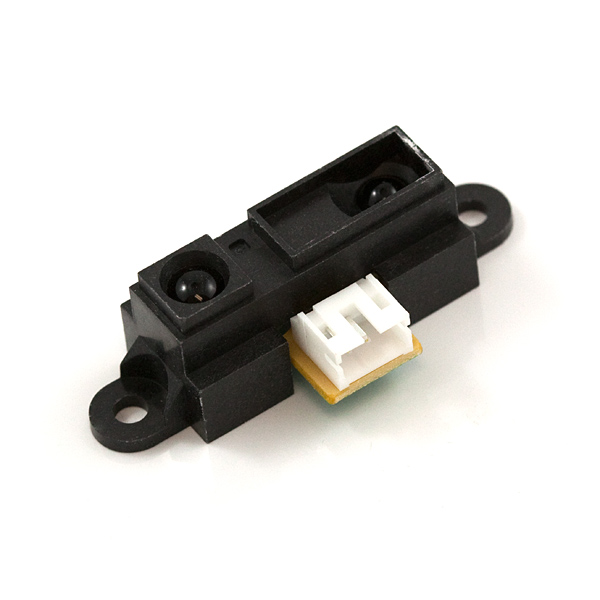
\includegraphics[width=0.5\textwidth]{figures/sensor}
	\caption{SHARP IR distance sensor}
	\label{fig:sensor}
\end{figure}
\section{Components choice and design implementation}
This unit is contains three main parts, a PSD (position sensitive detector), a IR-LED and a signal processing circuit. The sensor working principle is based on triangulation method (figure \ref{fig:sensorprinciple}).By using the triangulation method, the effects of environmental temperature, reflectivity of the the measured object affect the distance detection in a reduced scale. 

\begin{figure}[!ht]
	\centering
	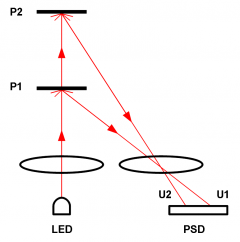
\includegraphics[width=0.5\textwidth]{figures/sensor_principle}
	\caption{Sensor working principle}
	\label{fig:sensorprinciple}
\end{figure}

The sensor requires DC power supply, and produces an analogue voltage output according to the measured distance. According to the data sheet, the operating supply voltage for the sensor is 4.5-5.5 V. Our main board provides a 5 V power supply. We decided to use this value for the $V_{cc}$ of the sensor.

The output according to the data sheet should under usual operating conditions range from 0 to peak around 3.1 V. 
We tested the sensor directly with the 5 V on the input and observed the results of measurements with different surfaces. The $V_{o}$ output values were very similar between each of the measured surfaces. The maximum value was moving around 3.2 V but sometimes we measured higher values above 3.8 V. The output signal tends to be very stable, without ripple. We were considering to add an averaging or low-pass filter in case of noise, but we had assumed that this was not necessary. To stabilize potential ripple on the sensor power supply we added a 10 $\mu F$  tantalum capacitor according to the data sheet. 


\begin{figure}[!ht]
	\centering
	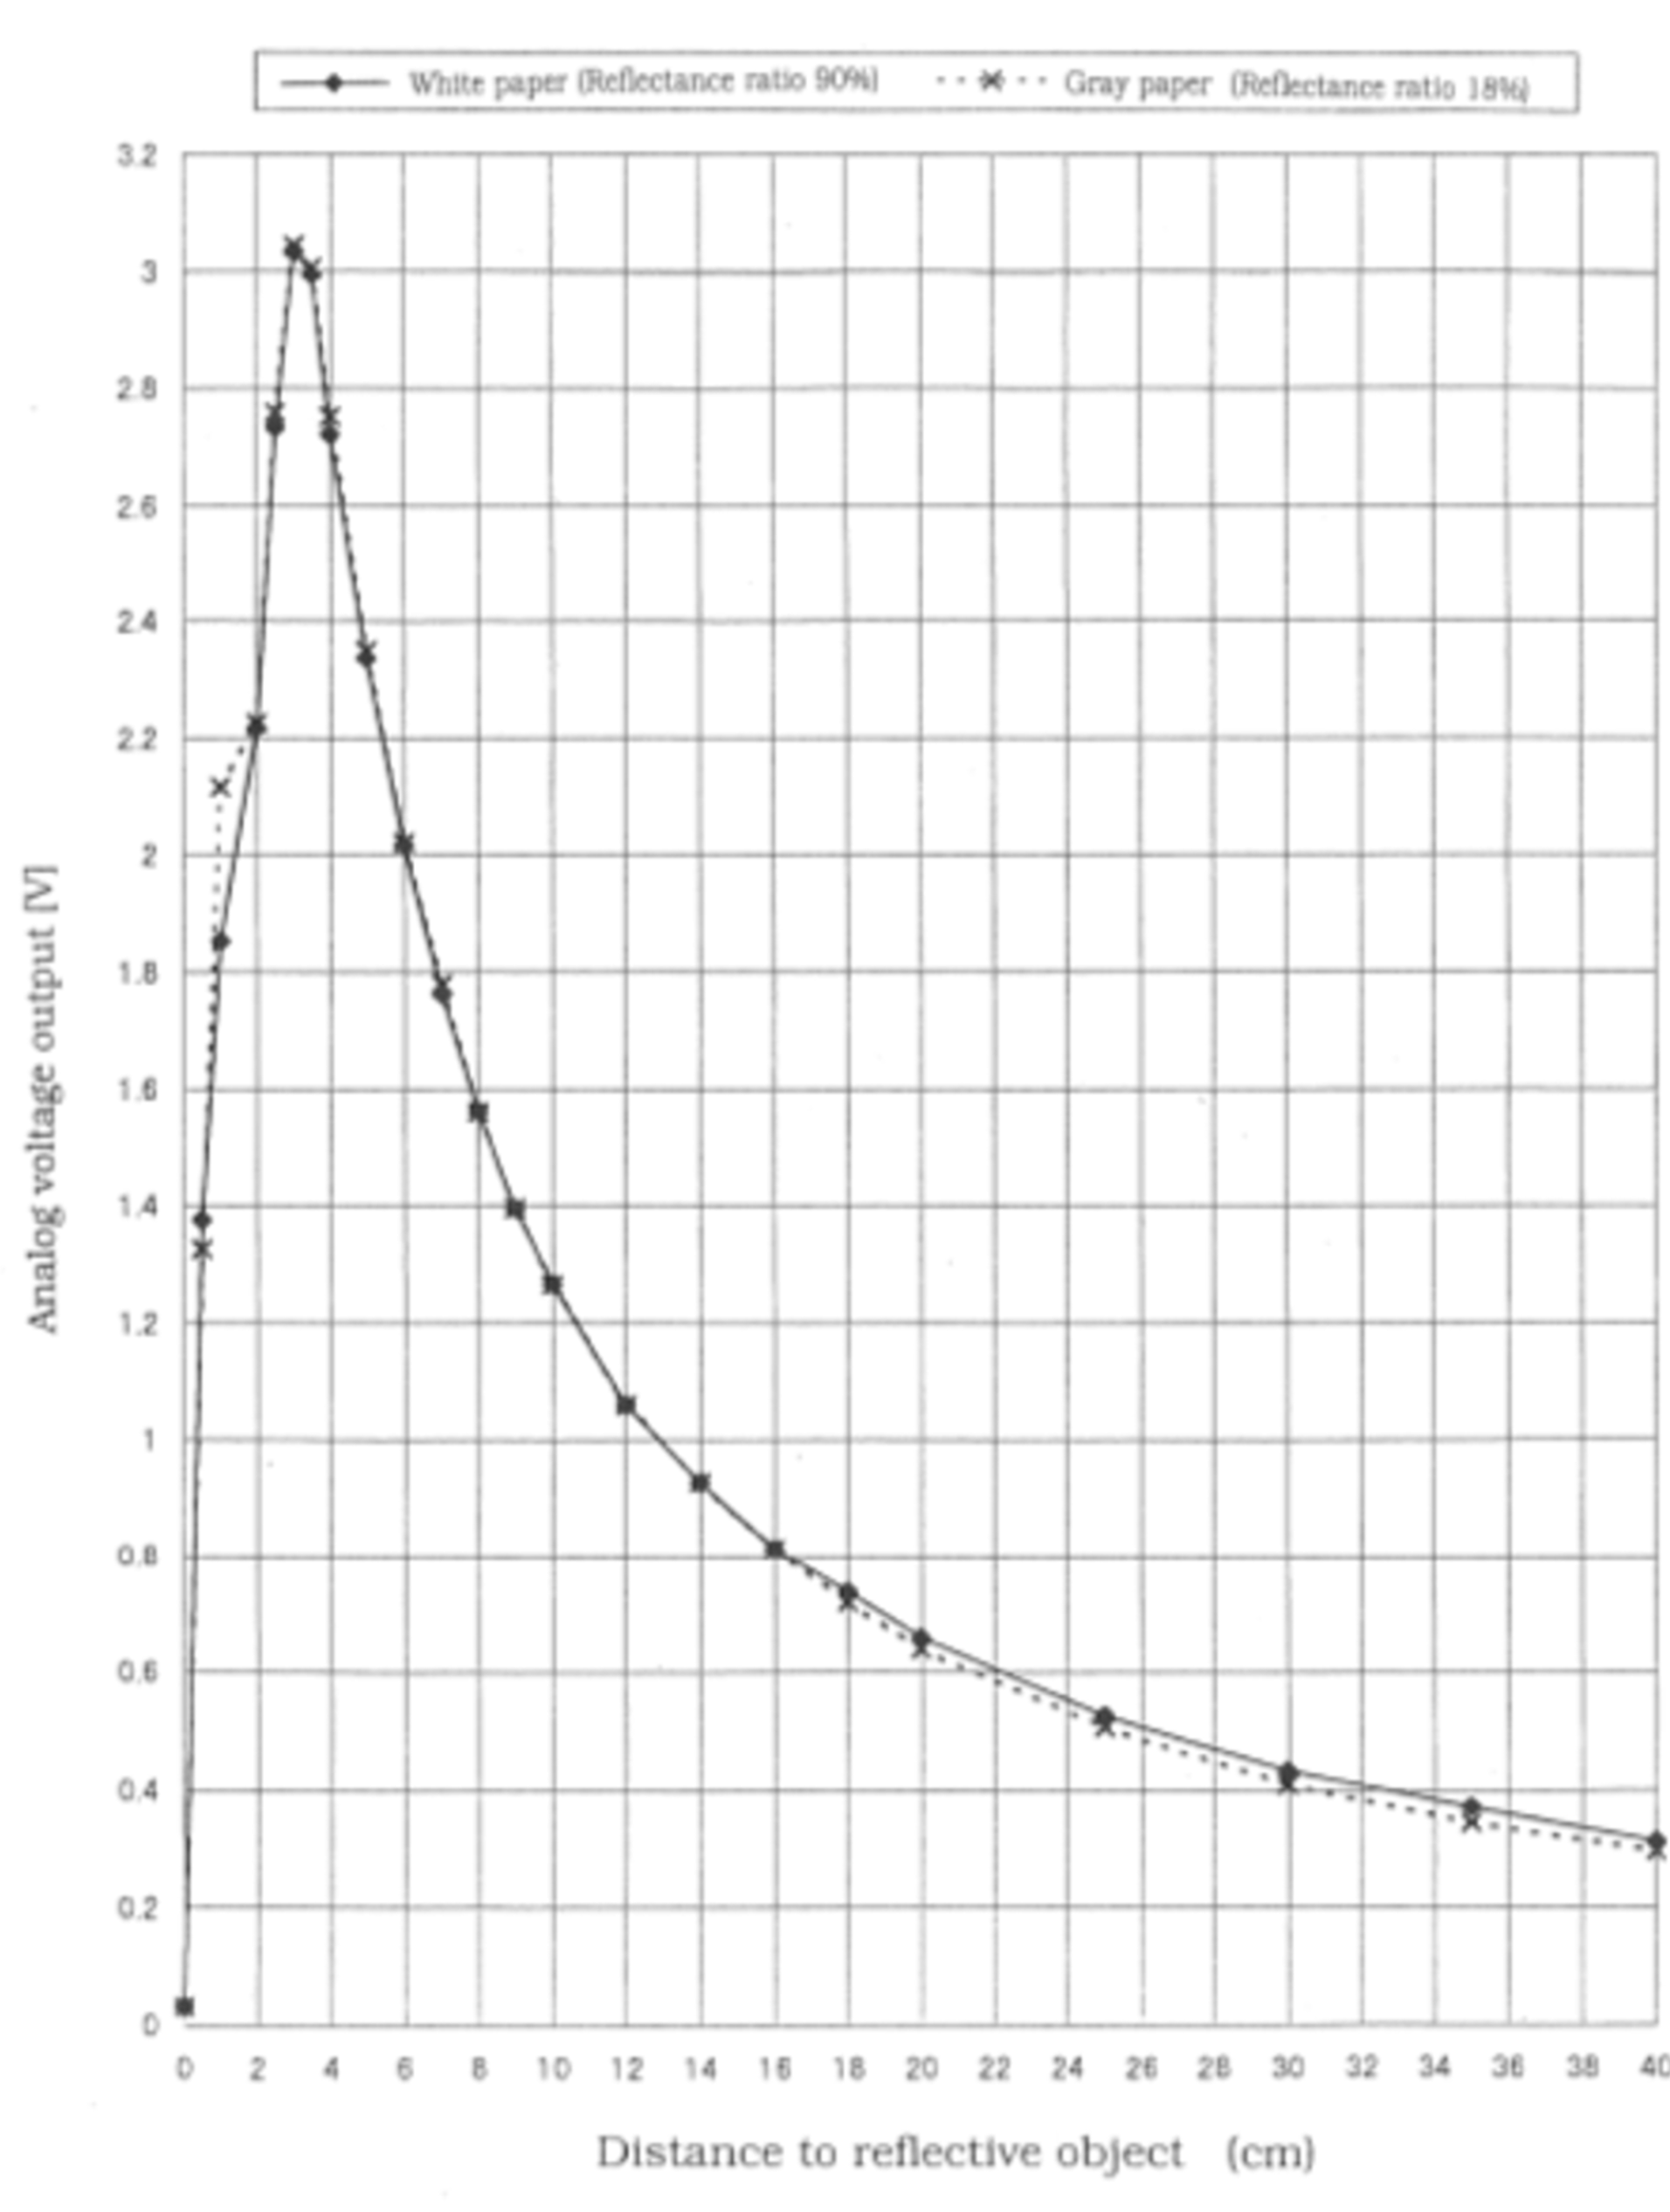
\includegraphics[width=0.5\textwidth]{figures/sensorchar}
	\caption{Distance sensor output characteristics }
	\label{fig:sensorchar}
\end{figure}


To interface the sensor output with the FPGA we need to convert the analog signal to digital. For this purpose we chose $TCL 1549CP$ 10-Bit A/D  successive-approximation Analog/Digital converter. As we are using ADC with the same reference value and $V_{cc}$ 5 V. This is a reasonable easy solution saving space and additional components. As an analog input to the ADC we put the $V_{o}$ from the sensor. At first we tried to use an non-inverting amplifier to stretch the sensor output voltage to 0-5 V. We managed to build this amplifying circuit but it appeared rather unnecessary as this way we only increase the signal range of sensor $V_{o}$ for about 1 V. The difference is not significant and doesn't have a big impact on the final control system. 

To connect the output of ADC to the FPGA it is necessary to  lower the 5 V output from ADC to 3.3 V input of FPGA.  We chose to use a simple zener clamp (figure \ref{fig:zener}) that works like a voltage regulator \cite{inventors}, \cite{tricks}, which a bit slower, but stable and robust enough to perform under given conditions. When the $V_{in}$  is below diode's breakdown voltage, the $V_{o} = V_{out} $. When the voltage is above this value, the diode draws as much current as necessary to keep $V_{out}$ at the level breakdown voltage (for us 3.3 V). 
We use a BZX79 - C3V3 Zener diode which working voltage is around 3.3 V. The resistor limits possible high currents through the diode to protect it. It is very recommended to be used. We tested the circuit with a 1 $k\Omega$ resistor. $I_{zener}=\frac{V_{in}-V_{out}}{R}=\frac{5-3.3}{1000}= 1.7 mA$  which is a value low enough. 

\begin{figure}[!ht]
	\centering
	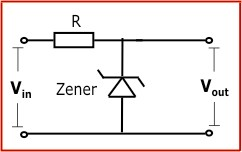
\includegraphics[width=0.5\textwidth]{figures/zener}
	\caption{Zener voltage clamper}
	\label{fig:zener}
\end{figure}


\newpage
\section{Conclusions}
After testing every component and interfacing the sensor with FPGA through the ADC we printed to separate PCBs, one which is mounted on the main board (containing the ADC and zener diode clamper) and one which contains the distance sensor. These two PCBs are connected together. 

\chapter{Chasis and mounting}
\label{chap:Chassis}

In the final part we designed a chasis and printed it on a 3D printer. This chasis
was aimed to be as light as possible for enabling the robot to perform better and as much mechanically robust as necessary. The chasis can be seen here:
\\It is a planar platform on which we mounted the printed boards (2 H-bridge boards, 1 main board, 1 logical gate board, and 1 sensor board). The motors are mounted in two specially designed holes to stay fixed while on duty. 

\chapter{notes}
We measured the H-bridge, with 12 V Vcc and 3.3 V on the transistor base , on the motor pins were 11.3 V. Its good
We tested also NAND and AND circuit to prevent 1,1 state on the h-bridge, but we got problems with pwm, then current so we decided for a simpler solution. DIR and SPEED.

Insert boards and schematics - Michelangelo
Insert remaining pictures into H-bridge chapter - Michelangelo
Improve switching regulator part
ADD references
ADD introduction and
Insert my camera photos
